\documentclass[a4paper]{article}

\def\npart {II}
\def\nterm {Michaelmas}
\def\nyear {2015}
\def\nlecturer {H. Wilton}
\def\ncourse {Algebraic Topology}
\def\nnotready {}

% Imports
\ifx \nextra \undefined
  \usepackage[pdftex,
    hidelinks,
    pdfauthor={Dexter Chua},
    pdfsubject={Cambridge Maths Notes: Part \npart\ - \ncourse},
    pdftitle={Part \npart\ - \ncourse},
  pdfkeywords={Cambridge Mathematics Maths Math \npart\ \nterm\ \nyear\ \ncourse}]{hyperref}
  \title{Part \npart\ - \ncourse}
\else
  \usepackage[pdftex,
    hidelinks,
    pdfauthor={Dexter Chua},
    pdfsubject={Cambridge Maths Notes: Part \npart\ - \ncourse\ (\nextra)},
    pdftitle={Part \npart\ - \ncourse\ (\nextra)},
  pdfkeywords={Cambridge Mathematics Maths Math \npart\ \nterm\ \nyear\ \ncourse\ \nextra}]{hyperref}

  \title{Part \npart\ - \ncourse \\ {\Large \nextra}}
\fi

\author{Lectured by \nlecturer \\\small Notes taken by Dexter Chua}
\date{\nterm\ \nyear}

\usepackage{alltt}
\usepackage{amsfonts}
\usepackage{amsmath}
\usepackage{amssymb}
\usepackage{amsthm}
\usepackage{booktabs}
\usepackage{caption}
\usepackage{enumitem}
\usepackage{fancyhdr}
\usepackage{graphicx}
\usepackage{mathtools}
\usepackage{microtype}
\usepackage{multirow}
\usepackage{pdflscape}
\usepackage{pgfplots}
\usepackage{siunitx}
\usepackage{tabularx}
\usepackage{tikz}
\usepackage{tkz-euclide}
\usepackage[normalem]{ulem}
\usepackage[all]{xy}

\pgfplotsset{compat=1.12}

\pagestyle{fancyplain}
\lhead{\emph{\nouppercase{\leftmark}}}
\ifx \nextra \undefined
  \rhead{
    \ifnum\thepage=1
    \else
      \npart\ \ncourse
    \fi}
\else
  \rhead{
    \ifnum\thepage=1
    \else
      \npart\ \ncourse\ (\nextra)
    \fi}
\fi
\usetikzlibrary{arrows}
\usetikzlibrary{decorations.markings}
\usetikzlibrary{decorations.pathmorphing}
\usetikzlibrary{positioning}
\usetikzlibrary{fadings}
\usetikzlibrary{intersections}
\usetikzlibrary{cd}

\newcommand*{\Cdot}{\raisebox{-0.25ex}{\scalebox{1.5}{$\cdot$}}}
\newcommand {\pd}[2][ ]{
  \ifx #1 { }
    \frac{\partial}{\partial #2}
  \else
    \frac{\partial^{#1}}{\partial #2^{#1}}
  \fi
}

% Theorems
\theoremstyle{definition}
\newtheorem*{aim}{Aim}
\newtheorem*{axiom}{Axiom}
\newtheorem*{claim}{Claim}
\newtheorem*{cor}{Corollary}
\newtheorem*{defi}{Definition}
\newtheorem*{eg}{Example}
\newtheorem*{fact}{Fact}
\newtheorem*{law}{Law}
\newtheorem*{lemma}{Lemma}
\newtheorem*{notation}{Notation}
\newtheorem*{prop}{Proposition}
\newtheorem*{thm}{Theorem}

\renewcommand{\labelitemi}{--}
\renewcommand{\labelitemii}{$\circ$}
\renewcommand{\labelenumi}{(\roman{*})}

\let\stdsection\section
\renewcommand\section{\newpage\stdsection}

% Strike through
\def\st{\bgroup \ULdepth=-.55ex \ULset}

% Maths symbols
\newcommand{\bra}{\langle}
\newcommand{\ket}{\rangle}

\newcommand{\N}{\mathbb{N}}
\newcommand{\Z}{\mathbb{Z}}
\newcommand{\Q}{\mathbb{Q}}
\renewcommand{\H}{\mathbb{H}}
\newcommand{\R}{\mathbb{R}}
\newcommand{\C}{\mathbb{C}}
\newcommand{\Prob}{\mathbb{P}}
\renewcommand{\P}{\mathbb{P}}
\newcommand{\E}{\mathbb{E}}
\newcommand{\F}{\mathbb{F}}
\newcommand{\cU}{\mathcal{U}}
\newcommand{\RP}{\mathbb{RP}}
\newcommand{\CP}{\mathbb{CP}}

\newcommand{\ph}{\,\cdot\,}

\DeclareMathOperator{\sech}{sech}
\DeclareMathOperator{\cosech}{cosech}
\DeclareMathOperator{\cosec}{cosec}

\DeclareMathOperator{\covol}{covol}
\DeclareMathOperator{\vol}{vol}

\let\Im\relax
\let\Re\relax
\DeclareMathOperator{\Im}{Im}
\DeclareMathOperator{\Re}{Re}
\DeclareMathOperator{\im}{im}
\DeclareMathOperator{\image}{image}
\DeclareMathOperator{\Ann}{Ann}

\DeclareMathOperator*{\res}{res}
\DeclareMathOperator{\Res}{Res}
\DeclareMathOperator{\Ind}{Ind}

\DeclareMathOperator{\tr}{tr}
\DeclareMathOperator{\diag}{diag}
\DeclareMathOperator{\rank}{rank}
\DeclareMathOperator{\card}{card}
\DeclareMathOperator{\spn}{span}
\DeclareMathOperator{\adj}{adj}

\DeclareMathOperator{\erf}{erf}
\DeclareMathOperator{\erfc}{erfc}

\DeclareMathOperator{\ord}{ord}
\DeclareMathOperator{\Sym}{Sym}

\DeclareMathOperator{\sgn}{sgn}
\DeclareMathOperator{\orb}{orb}
\DeclareMathOperator{\stab}{stab}
\DeclareMathOperator{\ccl}{ccl}

\DeclareMathOperator{\lcm}{lcm}
\DeclareMathOperator{\hcf}{hcf}

\DeclareMathOperator{\Int}{Int}
\DeclareMathOperator{\id}{id}

\DeclareMathOperator{\betaD}{beta}
\DeclareMathOperator{\gammaD}{gamma}
\DeclareMathOperator{\Poisson}{Poisson}
\DeclareMathOperator{\binomial}{binomial}
\DeclareMathOperator{\multinomial}{multinomial}
\DeclareMathOperator{\Bernoulli}{Bernoulli}
\DeclareMathOperator{\like}{like}

\DeclareMathOperator{\var}{var}
\DeclareMathOperator{\cov}{cov}
\DeclareMathOperator{\bias}{bias}
\DeclareMathOperator{\mse}{mse}
\DeclareMathOperator{\corr}{corr}

\DeclareMathOperator{\otp}{otp}
\DeclareMathOperator{\dom}{dom}

\DeclareMathOperator{\Root}{Root}
\DeclareMathOperator{\supp}{supp}
\DeclareMathOperator{\rel}{rel}
\DeclareMathOperator{\Hom}{Hom}
\DeclareMathOperator{\Aut}{Aut}
\DeclareMathOperator{\Gal}{Gal}
\DeclareMathOperator{\Mat}{Mat}
\DeclareMathOperator{\End}{End}
\DeclareMathOperator{\Char}{char}
\DeclareMathOperator{\ev}{ev}
\DeclareMathOperator{\St}{St}
\DeclareMathOperator{\Lk}{Lk}
\DeclareMathOperator{\disc}{disc}
\DeclareMathOperator{\Isom}{Isom}
\DeclareMathOperator{\length}{length}
\DeclareMathOperator{\energy}{energy}
\DeclareMathOperator{\area}{area}
\DeclareMathOperator{\Syl}{Syl}
\DeclareMathOperator{\cl}{cl}
\DeclareMathOperator{\fix}{fix}

\newcommand{\GL}{\mathrm{GL}}
\newcommand{\SL}{\mathrm{SL}}
\newcommand{\PGL}{\mathrm{PGL}}
\newcommand{\PSL}{\mathrm{PSL}}
\newcommand{\PSU}{\mathrm{PSU}}
\newcommand{\Or}{\mathrm{O}}
\newcommand{\SO}{\mathrm{SO}}
\newcommand{\U}{\mathrm{U}}
\newcommand{\SU}{\mathrm{SU}}

\renewcommand{\d}{\mathrm{d}}
\newcommand{\D}{\mathrm{D}}

\tikzset{->/.style = {decoration={markings,
                                  mark=at position 1 with {\arrow[scale=2]{latex'}}},
                      postaction={decorate}}}
\tikzset{<-/.style = {decoration={markings,
                                  mark=at position 0 with {\arrowreversed[scale=2]{latex'}}},
                      postaction={decorate}}}
\tikzset{<->/.style = {decoration={markings,
                                   mark=at position 0 with {\arrowreversed[scale=2]{latex'}},
                                   mark=at position 1 with {\arrow[scale=2]{latex'}}},
                       postaction={decorate}}}
\tikzset{->-/.style = {decoration={markings,
                                   mark=at position #1 with {\arrow[scale=2]{latex'}}},
                       postaction={decorate}}}
\tikzset{-<-/.style = {decoration={markings,
                                   mark=at position #1 with {\arrowreversed[scale=2]{latex'}}},
                       postaction={decorate}}}

\tikzset{circ/.style = {fill, circle, inner sep = 0, minimum size = 3}}
\tikzset{mstate/.style={circle, draw, blue, text=black, minimum width=0.7cm}}

\definecolor{mblue}{rgb}{0.2, 0.3, 0.8}
\definecolor{morange}{rgb}{1, 0.5, 0}
\definecolor{mgreen}{rgb}{0.1, 0.4, 0.2}
\definecolor{mred}{rgb}{0.5, 0, 0}

\def\drawcirculararc(#1,#2)(#3,#4)(#5,#6){%
    \pgfmathsetmacro\cA{(#1*#1+#2*#2-#3*#3-#4*#4)/2}%
    \pgfmathsetmacro\cB{(#1*#1+#2*#2-#5*#5-#6*#6)/2}%
    \pgfmathsetmacro\cy{(\cB*(#1-#3)-\cA*(#1-#5))/%
                        ((#2-#6)*(#1-#3)-(#2-#4)*(#1-#5))}%
    \pgfmathsetmacro\cx{(\cA-\cy*(#2-#4))/(#1-#3)}%
    \pgfmathsetmacro\cr{sqrt((#1-\cx)*(#1-\cx)+(#2-\cy)*(#2-\cy))}%
    \pgfmathsetmacro\cA{atan2(#2-\cy,#1-\cx)}%
    \pgfmathsetmacro\cB{atan2(#6-\cy,#5-\cx)}%
    \pgfmathparse{\cB<\cA}%
    \ifnum\pgfmathresult=1
        \pgfmathsetmacro\cB{\cB+360}%
    \fi
    \draw (#1,#2) arc (\cA:\cB:\cr);%
}
\newcommand\getCoord[3]{\newdimen{#1}\newdimen{#2}\pgfextractx{#1}{\pgfpointanchor{#3}{center}}\pgfextracty{#2}{\pgfpointanchor{#3}{center}}}

\def\Xint#1{\mathchoice
   {\XXint\displaystyle\textstyle{#1}}%
   {\XXint\textstyle\scriptstyle{#1}}%
   {\XXint\scriptstyle\scriptscriptstyle{#1}}%
   {\XXint\scriptscriptstyle\scriptscriptstyle{#1}}%
   \!\int}
\def\XXint#1#2#3{{\setbox0=\hbox{$#1{#2#3}{\int}$}
     \vcenter{\hbox{$#2#3$}}\kern-.5\wd0}}
\def\ddashint{\Xint=}
\def\dashint{\Xint-}


\begin{document}
\maketitle
{\small
\noindent\textbf{The fundamental group}\\
Homotopy of continuous functions and homotopy equivalence between topological spaces. The fundamental group of a space, homomorphisms induced by maps of spaces, change of base point, invariance under homotopy equivalence.\hspace*{\fill} [3]

\vspace{10pt}
\noindent\textbf{Covering spaces}\\
Covering spaces and covering maps. Path-lifting and homotopy-lifting properties, and their application to the calculation of fundamental groups. The fundamental group of the circle; topological proof of the fundamental theorem of algebra. *Construction of the universal covering of a path-connected, locally simply connected space*. The correspondence between connected coverings of $X$ and conjugacy classes of subgroups of the fundamental group of $X$.\hspace*{\fill} [5]

\vspace{10pt}
\noindent\textbf{The Seifert-Van Kampen theorem}\\
Free groups, generators and relations for groups, free products with amalgamation. Statement *and proof* of the Seifert-Van Kampen theorem. Applications to the calculation of fundamental groups.\hspace*{\fill} [4]

\vspace{10pt}
\noindent\textbf{Simplicial complexes}\\
Finite simplicial complexes and subdivisions; the simplicial approximation theorem.\hspace*{\fill} [3]

\vspace{10pt}
\noindent\textbf{Homology}\\
Simplicial homology, the homology groups of a simplex and its boundary. Functorial properties for simplicial maps. *Proof of functoriality for continuous maps, and of homotopy invariance*.\hspace*{\fill} [4]

\vspace{10pt}
\noindent\textbf{Homology calculations}\\
The homology groups of $S^n$, applications including Brouwer's fixed-point theorem. The Mayer-Vietoris theorem. *Sketch of the classification of closed combinatorical surfaces*; determination of their homology groups. Rational homology groups; the Euler-Poincar\'e characteristic and the Lefschetz fixed-point theorem.\hspace*{\fill} [5]}

\tableofcontents

\setcounter{section}{-1}
\section{Introduction}
In topology, a typical problem is that we have two spaces $X$ and $Y$, and we want to know if $X\simeq Y$, ie. if $X$ and $Y$ are homeomorphic. If they are homeomorphic, we can easily show this by writing down a homeomorphism. But what if they are not? How can we prove that two spaces are not homeomorphic?

For example, are $\R^m$ and $\R^n$ homeomorphic (for $m\not= n$)? Intuitively, they should not be, since they have different dimensions, and in fact they are. But how can we actually prove this?

The idea of algebraic topology is to translate these non-existence problems in topology to non-existence problems in algebra. It turns out we are much better at algebra than topology. It is \emph{much} easier to show that two groups are not isomorphic.

While the statement that $\R^m \not\simeq \R^n$ for $n \not= m$ is intuitively obvious, algebraic topology can be used to prove some less obvious results.

Let $D^n$ be the $n$ dimensional unit disk, and $S^{n - 1}$ be the $n-1$ dimensional unit sphere. We will be able to show that there is no continuous map $F: D^n \to S^{n - 1}$ such that the composition
\[
  \begin{tikzcd}
    S^{n - 1} \ar[r, hook] & D^n \ar[r, "F"] & S^{n - 1}
  \end{tikzcd}
\]
is the identity, where the first arrow is the inclusion map. Alternatively, this says that we cannot continuously map the disk onto the boundary sphere such that the boundary sphere is fixed by the map.

Using algebraic topology, we can translate this statement into an algebraic statement: there is no homomorphism $F: \{0\} \to \Z$ such that
\[
  \begin{tikzcd}
    \Z \ar[r, hook] & \{0\} \ar[r, "F"] & \Z
  \end{tikzcd}
\]
is the identity. This is something we can prove in 5 seconds.

By translating a non-existence problem of a continuous map to a non-existence problem of a homomorphism, we have made our life much easier.

In algebraic topology, we will be developing a lot of machinery to do this sort of translation. However, this machinery is not easy. It will take some hard work, and will be rather tedious and boring at the beginning. So keep in mind that the point of all that hard work is to prove all these interesting theorems.

In case you are completely uninterested in topology, and don't care if $\R^m$ and $\R^n$ are homeomorphic, further applications of algebraic topology include \emph{solving equations}. For example, we will be able to prove the fundamental theorem of algebra, as well as Brouwer's fixed point theorem (which says that every continuous function from $D^2 \to D^2$ has a fixed point). If you are not interested in these as well, you may as well drop this course.

\section{Definitions}
\subsection{Some recollections and conventions}
We will start with some preliminary definitions and conventions.

\begin{defi}[Map]
  In this course, the word \emph{map} will always refer to continuous maps. We are doing topology, and never care about non-continuous functions.
\end{defi}

We are going to build a lot of continuous maps in algebraic topology. To do so, we will often need to glue maps together. The \emph{glueing lemma} tells us that this works.
\begin{lemma}[Glueing lemma]
  If $f: X\to Y$ is a function of topological spaces, $X = C\cup K$, $C$ and $K$ are both closed, then $f$ is continuous if and only if the restrictions $f|_C$ and $f|_K$are continuous.
\end{lemma}
The proof is easy from the definition of continuous maps.

\subsection{Cell complexes}
In general, we can construct some really horrible topological spaces. Even if we require them to be compact, Hausdorff etc, we can often still produce really ugly topological spaces. In algebraic topology, we will often restrict our attention to some nice topological spaces, known as \emph{cell complexes}.

To build cell complexes, we are not just glueing maps, but spaces.

\begin{defi}[Cell attachment]
  Fora a space $X$, and a map $f: S^{n - 1}\to X$, the space obtained by \emph{attaching an $n$-cell} to $X$ along $f$ is
  \[
    X\cup_{f}D^n = (X\sqcup D^N)/{\sim},
  \]
  where the equivalence relation $\sim$ is the equivalence relation generated by $x\sim f(x)$ for all $x\in S^{n - 1}\subseteq D^n$.

  Intuitively, a map $f: S^{n - 1}\to X$ is just picks out a subset $X$ that looks like the sphere. So we are just sticking a disk onto $X$ by attaching the boundary of the disk onto a sphere within $X$.
  \begin{center}
    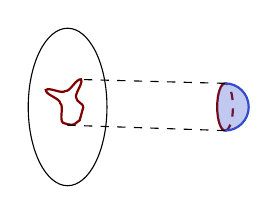
\begin{tikzpicture}
      \draw ellipse (0.5 and 1);

      \draw [thick, mred, decorate, decoration={snake}] circle [radius=0.2];

      \draw [thick, mred] (2, 0.3) arc (90:270:0.1 and 0.3);
      \draw [dashed, thick, mred] (2, -0.3) arc (270:450:0.1 and 0.3);

      \fill [mblue, opacity=0.3] (2, 0.3) arc (90:270:0.1 and 0.3) arc (270:450:0.3);
      \draw [thick, mblue] (2, -0.3) arc (270:450:0.3);

      \draw [dashed] (2, 0.3) -- (0.12, 0.35);
      \draw [dashed] (2, -0.3) -- (-0.05, -0.23);
    \end{tikzpicture}
  \end{center}
  % insert diagram.
\end{defi}

\begin{defi}[Cell complex]
  A (finite) \emph{cell complex} is a space $X$ obtained by
  \begin{enumerate}
    \item Start with a discrete finite set $X^{(0)}$.
      \begin{center}
        \begin{tikzpicture}
          \node [circ] at (0, 0) {};
          \node [circ] at (-1, -1.2) {};
          \node [circ] at (1, -1) {};
          \node [circ] at (0.3, -2) {};
        \end{tikzpicture}
      \end{center}
    \item Given $X^{n - 1}$, for $X^n$ by taking a finite set of maps $\{f_\alpha: S^{n - 1} \to X^{(n - 1)}\}$  by attaching $n$-cells along the $f_\alpha$:
      \[
        X^{(n)} = \left(X^{(n - 1)}\sqcup \bigsqcup_\alpha D_{\alpha}^N\right)/\{x\sim f_\alpha(x)\}.
      \]
      For example, given the $X^{(0)}$ above, we can attach some loops and lines to obtain the following $X^{(1)}$
      \begin{center}
        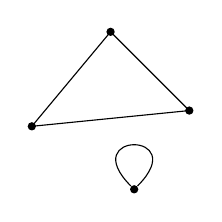
\begin{tikzpicture}
          \node [circ] at (0, 0) {};
          \node [circ] at (-1, -1.2) {};
          \node [circ] at (1, -1) {};
          \node [circ] (3) at (0.3, -2) {};

          \draw (0, 0) -- (-1, -1.2) -- (1, -1) -- (0, 0);
          \draw (3) edge [loop, looseness=30] (3);
        \end{tikzpicture}
      \end{center}
      We can add surfaces to obtain the following $X^{(2)}$
      \begin{center}
        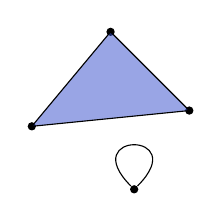
\begin{tikzpicture}
          \node [circ] at (0, 0) {};
          \node [circ] at (-1, -1.2) {};
          \node [circ] at (1, -1) {};
          \node [circ] (3) at (0.3, -2) {};

          \draw [fill = mblue, fill opacity=0.5] (0, 0) -- (-1, -1.2) -- (1, -1) -- (0, 0);
          \draw (3) edge [loop, looseness=30] (3);
        \end{tikzpicture}
      \end{center}
    \item Stop at some $X = X^{(k)}$. The minimum such $k$ is the \emph{dimension} of $X$.
  \end{enumerate}
  To define non-finite cell complexes, we just have to remove the words ``finite'' in the definition and remove the final condition.
\end{defi}

\begin{eg}
  The following is \emph{not} a cell complex: we take $\R^2$, and add a circle with radius $\frac{1}{2}$ and center $(0, \frac{1}{2})$. Then we add another circle with radius $\frac{1}{4}$ and center $(0, \frac{1}{4})$, then a circle with radius $\frac{1}{8}$ and center $(0, \frac{1}{8})$ etc. We obtain something like
  \begin{center}
    \begin{tikzpicture}[scale=2]
      \draw (0, 0.5) circle [radius=0.5];
      \draw (0, 0.25) circle [radius=0.25];
      \draw (0, 0.125) circle [radius = 0.125];
      \draw (0, 0.0625) circle [radius = 0.0625];
      \draw [gray] (-2, 0) -- (2, 0);

      \node [circ, mblue] at (0, 1) {};
      \node [circ, mblue] at (0, 0.5) {};
      \node [circ, mblue] at (0, 0.25) {};
      \node [circ, mblue] at (0, 0.125) {};
    \end{tikzpicture}
  \end{center}
  This is known as the \emph{Hawaiian Earring}.

  Why is this not an (infinite) cell complex? We did obtain it by attaching 1-cells to the single point $(0, 0)$. However, when attaching cells to a cell complex, the cells should not be ``close'' to each other. They are completely separated from each other apart from touching at the origin. However, here the circles clump together at the origin.

  In particular, if we take the following sequence $(0, 1), (0, \frac{1}{2}), (0, \frac{1}{4}), \cdots$, it converges to $(0, 0)$. If this were a cell complex, then this shouldn't happen because the cells are unrelated, and picking a point from each cell should not produce a convergent sequence (if you are not convinced, if we actually did produce by attaching cells, then note that during the attaching process, we needn't have attached them this way. We could have made it such that the $n$th cell has radius $n$. Then clearly picking the topmost point of each cell will not produce a convergent sequence).

  We will see that the Hawaiian Earring will be a counterexample to a lot of our theorems here.
\end{eg}

\section{Homotopy and the fundamental group}
This will be our first trick to translate topological spaces into groups.

\setcounter{subsection}{-1}
\subsection{Motivation}
Recall that we wanted to prove that $\R^n \not\simeq \R^m$ for $n\not= m$. Let's first do the simple case, where $m = 1, n = 2$. We want to show that $\R\not\simeq \R^2$.

This is not hard. We know that $\R$ is a line, while $\R^2$ is a plane. Let's try to remove a point from each of them.  If we remove a point from $\R$, the space stops being path connected. However, removing a point does not have this effect on $\R^2$. Since being path connected is a topological property, we have now showed that $\R$ and $\R^2$ are not homeomorphic.

Unfortunately, this does not extend very far. We cannot use this to show that $\R^2$ and $\R^3$ are not homeomorphic. What else can we do?

Notice that when we remove a point from $\R^2$, sure it is still connected, but something has changed.

Consider a circle containing the origin in $\R^2 \setminus \{0\}$. If the origin were there, we can keep shrinking the circle down until it becomes a point. However, we cannot do this if the origin is missing.
\begin{center}
  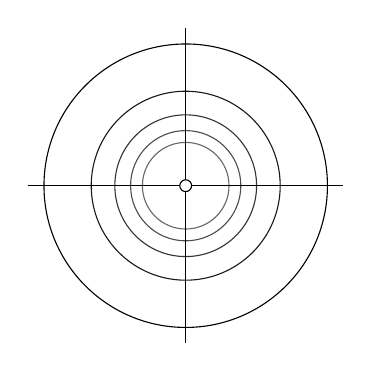
\begin{tikzpicture}
    \draw (-2, 0) -- (2, 0);
    \draw (0, -2) -- (0, 2);

    \draw [fill=white] circle [radius=0.075];
    \draw circle [radius=1.8];
    \draw [opacity=0.9] circle [radius=1.2];
    \draw [opacity=0.8] circle [radius=0.9];
    \draw [opacity=0.7] circle [radius=0.7];
    \draw [opacity=0.6] circle [radius=0.55];
  \end{tikzpicture}
\end{center}
The strategy now is to exploit the fact that $\R^2 \setminus \{0\}$ has circles which cannot be deformed to points.
\end{document}
